\section{Abstract}
\frame{\tableofcontents[currentsection, hideothersubsections]}

\begin{frame}
\frametitle{Abstract}

Problem:
\begin{itemize}
    \item for natural gradients, there is still NO way to \textbf{efficiently compute}
        the inverse of Fisher info matrix $F^{-1}$ (or its product with a vector)
\end{itemize}

Idea:
\begin{itemize}
    \item approximate $F^{-1}$ as block diagonal or block tridiagonal matrices
\end{itemize}

Result:
\begin{itemize}
    \item has cheap iterations like SGD
    \item needs fewer iterations than well-tuned SGD with momentum \\
        (not as few as Hessian-Free optimization (HFO))
\end{itemize}

\end{frame}

\begin{frame}
\frametitle{Abstract}
{\footnotesize
Left to right: \\
$\tilde{F}^{-1}$, its approximations $\breve{F}^{-1}$ (top) and $\hat{F}^{-1}$ (bottom), their absolute difference
}
\begin{figure}
    \centering
    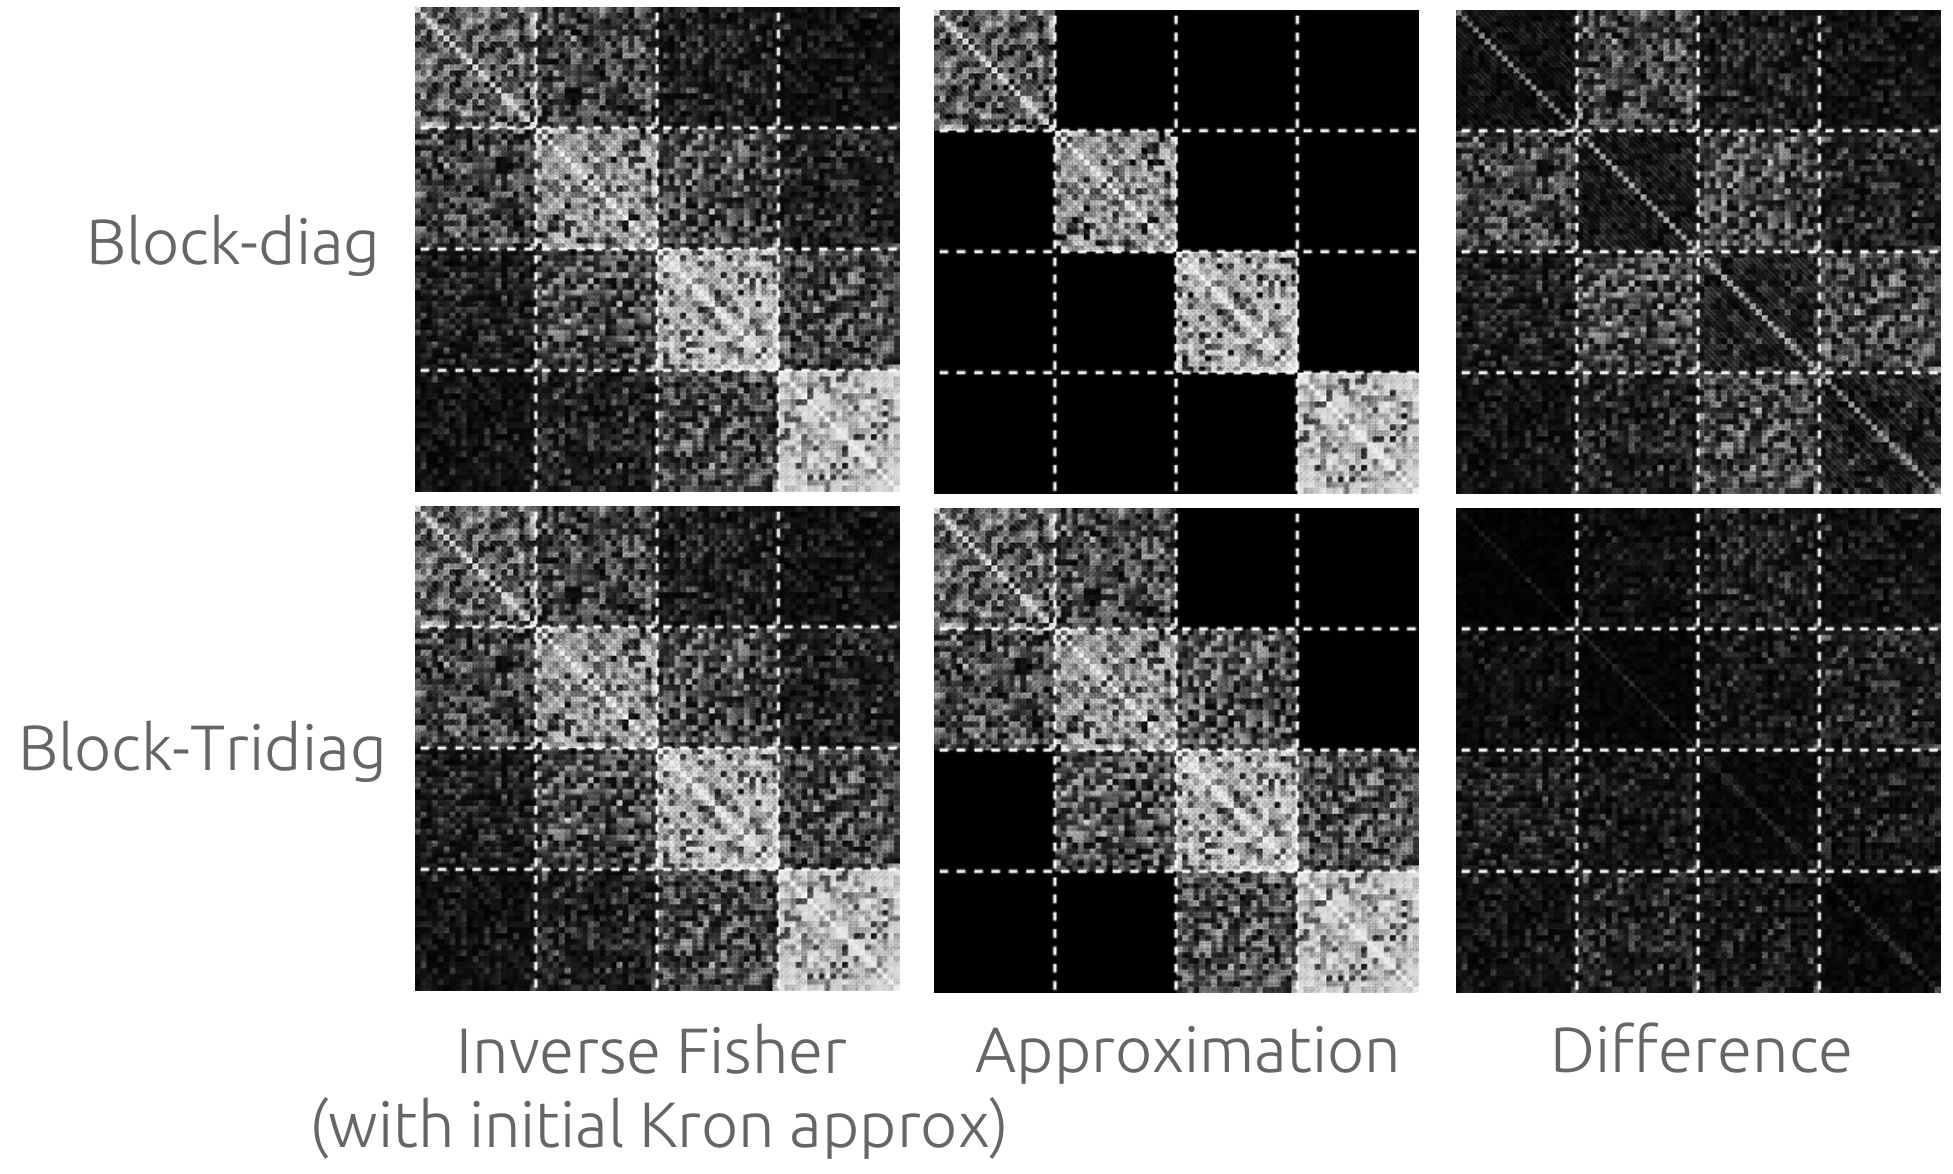
\includegraphics[scale=0.2]{kfac_12}
\end{figure}
(plotting absolute values of entries, dark means small)
\end{frame}

\begin{frame}
\frametitle{Abstract}
\begin{figure}
    \centering
    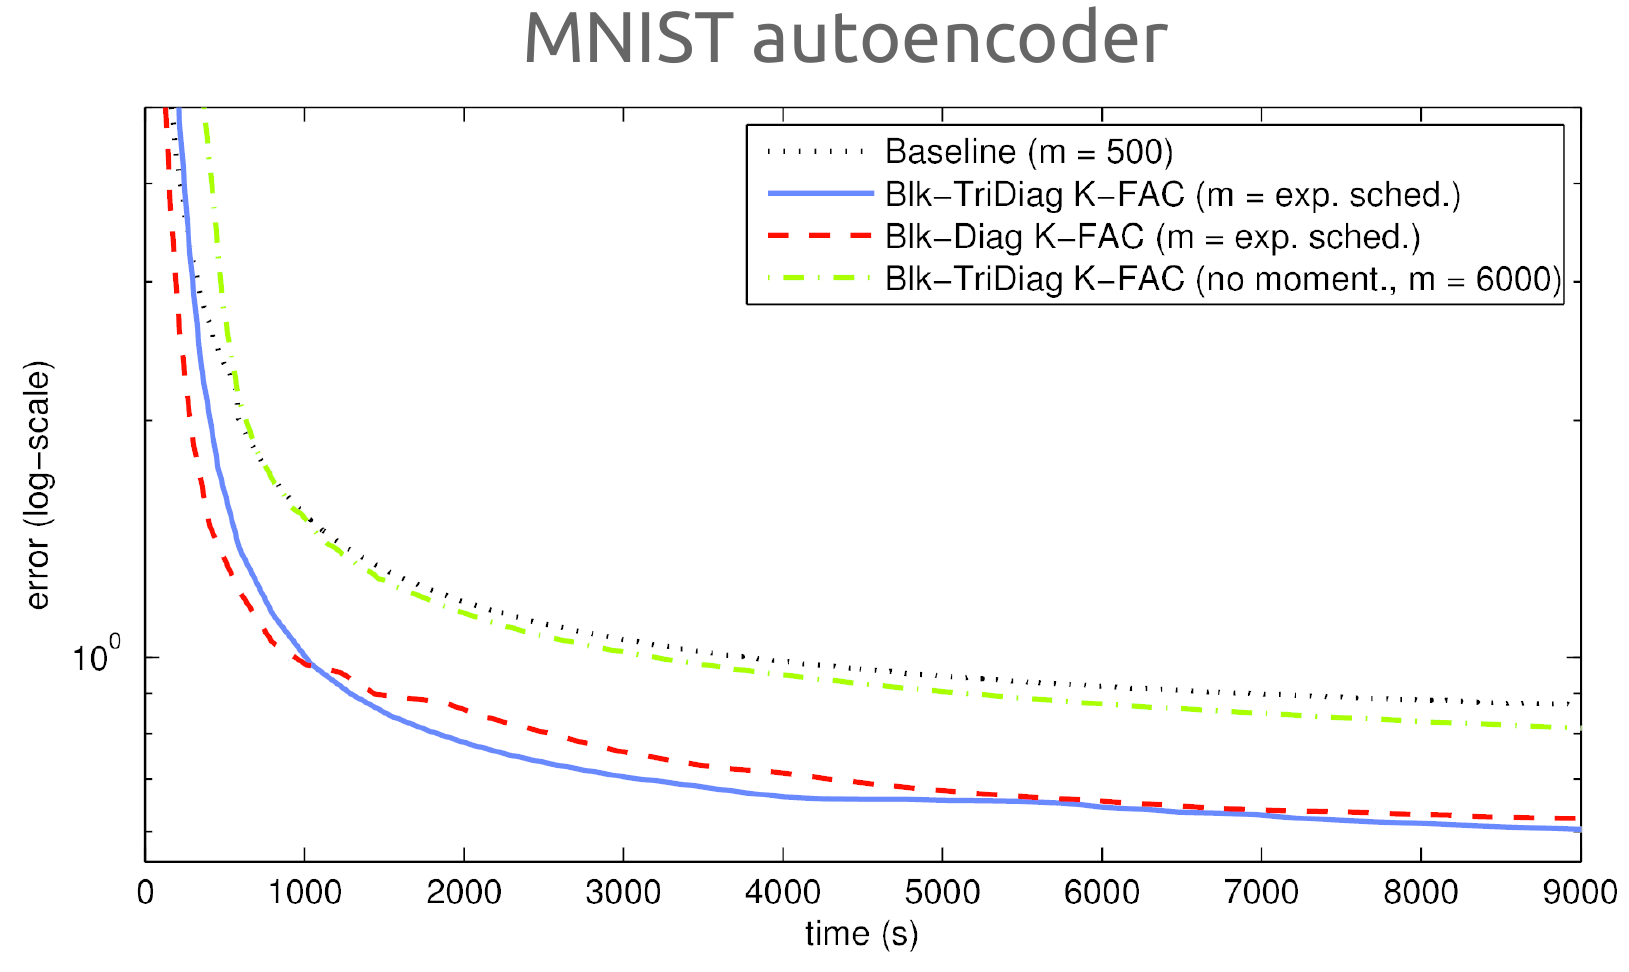
\includegraphics[scale=0.25]{mnist_autoencoder}
\end{figure}
(Baseline: well-tuned SGD with momentum)
\end{frame}
